\section{Die Peripherie}
\index{Peripherie}
Die UMach Maschine ist an einem \gls{Bussystem}\index{Bussystem} angeschlossen.
Dieses Bussystem enthält unter anderem Baukomponenten (Ports), an denen
peripherische Geräte physisch abgeschlossen sein können. Der
\gls{Speicher}\index{Speicher} der Maschine ist eine solche peripherische
Komponente, die an einem Port angeschlossen ist (am
Speicherport\index{Speicherport}). Eine andere peripherische Komponente ist das
Display, das an einem Video-Port des Busses angeschlossen ist. Eine weitere
Komponente ist die Tastatur. Wie diese Geräte intern funktionieren, weiß die
Maschine und das Bussystem nicht. Was sie \glqq wissen\grqq, ist dass diese
Geräte eine Reihe von Befehlen ausführen können (hauptsächlich \glqq
read/write\grqq\ oder \glqq load/store\grqq\ Befehle). Siehe dazu die Abbildung
\ref{fig:UMach-Bussystem} auf der Seite \pageref{fig:UMach-Bussystem}.

\begin{figure}
  \centering
  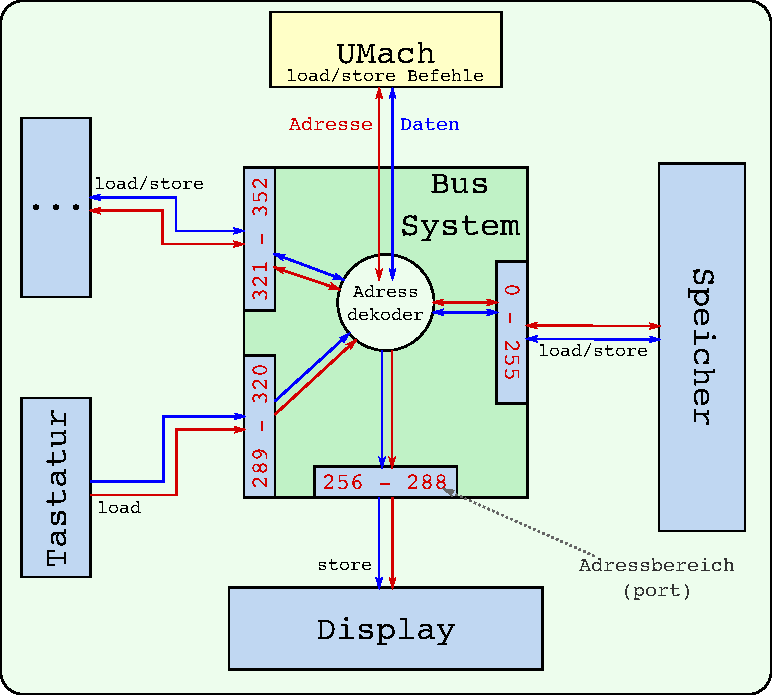
\includegraphics{img/UMach-Bus}
  \caption[Das UMach Bussystem]
          {Das UMach Bussystem verwendet eine einfache speicherbasierte
          Adressierung der peripherischen Komponenten, die an
          \glqq Memory Mapped I/O\grqq\ angelehnt ist. Jeder peripherischen
          Komponente wird vom Bussystem beim Hochfahren der Maschine einen
          eindeutigen Adressbereich zugeweisen.
          Die \glqq load/store\grqq\ Befehle der Maschine werden anhand deren
          Adressen vom Adressdekoder, der wie ein Demultiplexer funktioniert,
          an die entsprechende Komponente weitergeleitet. Die
          Adressbereiche $[0,255], [256,288]$ usw. sind nur als
          Beispiel gegeben. Der interne Speicher des Busses, der die
          Abbildungen der einzelen Ports auf Adressbereiche enthält, ist nicht
          dargestellt.}
  \label{fig:UMach-Bussystem}
\end{figure}



\subsection{Speicherbasierte Kommunikation}
\index{Speicherbasierte Kommunikation}

Die UMach Maschine kommuniziert nicht direkt mit den am Bus angeschlossenen
peripherischen Geräten, sondern sie verwendet dafür eine Art speicherbasierter
Kommunikation, die eine vereinfachte Form von \glqq Memory Mapped I/O\grqq\
darstellt.\index{Memory Mapped I/O} Wie dieses Verfahren funktioniert wird im
folgenden beschrieben.

Die Bus-Ports sind im Bussystem\index{Bussystem} physisch fest
eingebaut\footnote{Wir schließen nicht aus, dass unterschiedliche Realisierungen
der UMach Maschine unterschiedliche Ports haben.}. Deren Anzahl und
physikalische Eigenschaften sind zu jeder Zeit dem Bussystem bekannt. Zu diesen
physikalischen Eigenschaften zählt die Fähigkeit, bestimmte Befehle aufzunehmen
und auszuführen (mittels Port-lokalen Register, die Befehle speichern können),
sowie die Fähigkeit, Daten und Signale zu produzieren. Diese Eigenschaften
erlauben dem Bussystem, den Port als eine Speichereinheit zu betrachten. 

Da jeder Port als Speicher adressierbar ist, sieht das Bussystem jeden Port als
in einem einheitlichen, kontinuierlichen 32-Bit Speicherraum eingebettet (da
die UMach Maschine 32-Bit Adressen verwendet). Dieser gesamte Speicherraum ist
nicht physikalischer Natur, denn es gibt ja keinen Speicher, wo die Ports
eingebaut sind, sondern virtueller Natur: jedem Port wird vom Bussystem einen
festen Adressbereich innerhalb des gesamten Adressraums vergeben und bildet
somit einen Speicherunterraum\index{Speicherunterraum} innerhalt des gesamten
virtuellen Speicherraums.

Da an jedem Port Geräte mit unterschiedlichen physikalischen Eigenschaften
angeschlossen sein können, wie z.B. Speicher mit unterschiedlicher
Speicherkapazität, kann im Allgemeinen das Bussystem nicht im Vorraus festlegen,
wie groß ist der Adressbereich jedes einzelnen Ports. Diese Größe muss dynamisch
vom Bus festgelegt werden.

Beim Hochfahren der gesamten Maschine testet das Bussystem an jedem Port das
angeschlossene Gerät. Mittels eines einfachen Protokolls werden die konkrete
physikalische Eigenschaften des Geräts abgefragt. Nach der Abfrage und Testphase
hat das Bussystem in einem eigenen, internen Speicher eine Liste von Geräten und
deren Eigenschaften aufgebaut. Anhand dieser Liste legt das Bussystem fest, wie
groß ist der Adressbereich jedes einzelnen Ports. Die Abbildung
\ref{fig:UMach-Bussystem} auf der Seite \pageref{fig:UMach-Bussystem} zeigt sehr
vereinfacht eine solche Verteilung der Speicherunterräume auf die Adressbereiche
innerhalb des gesamten Speicherraums. Nach der Verteilung kann das Bussystem
jede 32-Bit Adresse einem bestimmten Port zuweisen.



\subsubsection{Adressierung}
\index{Peripherie!Adressierung}

Wie bereits oben erklärt, erstellt das Bussystem eine Abbildung der einzelnen
Bus-Ports auf Adressbereiche innerhalb eines 32-Bit Adressraums. Der Speicher
selbst belegt einen solchen Adressbereich.

Die Kommunikation der UMach Maschine mit den peripherischen Geräten besteht aus
Lade- und Speicherbefehle, die von der Maschine dem Bussystem übergeben werden
(siehe dazu den Abschnitt \ref{sec:Lade-Speicher-Instruktionen} ab der Seite
\pageref{sec:Lade-Speicher-Instruktionen}). Das Bussystem fängt diese Befehle in
seinem \gls{Adressdekoder} ab und entscheidet dort anhand der verwendeten
Adresse, für welchen Port sind die Befehle gemeint. Wenn das Bussystem den Port
identifiziert hat, leitet er den Befehl und die eventuellen Daten an den Port
weiter.
Siehe als Beispiel die Abbildung \ref{fig:UMach-Bussystem} auf der Seite
\pageref{fig:UMach-Bussystem}. In diesem Beispiel, möchte die Maschine Daten an
das Display senden, so verwendet sie einen Speicherbefehl (\glqq store\grqq),
der den Adressbereich des Displays verwendet. In der Abbildung
\ref{fig:UMach-Bussystem} wäre das eine Adresse im Bereich $[256, 288]$. Um den
Buchstaben 'A' auf dem Display anzuzeigen, sagt die Maschine dem Bussystem \glqq
speichere 'A' an die Adresse $256$\grqq. Um von der Tastatur zu lesen, sagt die
Maschine dem Bus \glqq lese aus der Adresse $289$\grqq.


Um die Adressbereiche bekannt zu machen, muss das Bussystem seinen eigenen
internen Speicher in den gesamten Adressbereich einbinden, und zwar an eine
feste Adresse. Somit kann der Programmierer der Maschine beim Start des
Programms die einzelnen Bereiche abfragen, verwenden und weiter unterteilen.











